\chapter{Dielectric Measurement Methods at Microwave Frequencies}\label{ch:methods}
\section{Introduction}
The ever increasing bandwidth requirements and the demand for better availability for mobile equipment is constantly pushing wireless communications to higher frequencies and greater efficiencies. Microwave engineering and material sciences have to keep pace with these recent developments. Dielectrics like microwave substrates or dielectric resonators play an important role in their efforts, since integrates circuits, printed circuits, filters and antennas - just to name a few applications - require well-characterised and understood dielectrics that perform well at microwave frequencies. Accurate characterisation of dielectrics is particularly important, as it could enable capabilities in rapid prototyping that have previously been unfeasible.

In the past, characterising dielectrics accurately at microwave frequencies has been relatively expensive and complicated. Out of this reason, both dielectric constant and loss tangent have often eluded measurement by scientists and engineers. While this applied to all dielectrics, it applied even more to low-loss dielectrics, which are often used as microwave substrates in integrated circuits and printed circuits. These materials typically have a very low dielectric loss, which can only be measured accurately with standing-wave methods (also called resonator methods). Unfortunately, many standing wave methods measure the permittivity only at one frequency (the resonant frequency) and very often the specimens have to be machined in order to measure them inside a resonator. The topic of this thesis is a standing-wave method that circumvents these two disadvantages of many standing-wave methods - the split-cylinder resonator method. 

The split-cylinder resonator is a very popular standing-wave dielectric measurement method, which was designed to operate at microwave frequencies. It uses a microwave cavity, which is split into two halves, an upper and a lower cavity. In between these two cavities a flat dielectric specimen can be placed, whose permittivity can then be measured by exciting one or multiple modes in this resonator. The specimen does not have to be prepared in any way before the measurement, as long as the specimen is sufficiently flat. The method itself was developed by Ermert \cite{ermert}, Guillon \cite{guillon}, Kobayashi \cite{kobayashi} and Kent \cite{kent1996}. Later, Janezic \cite{janezic} improved the method both in function and in accuracy. He derived a very efficient mode-matching model of the split-cylinder resonator that was widely adopted in the industry. Today, the measurement method is both an IPC standard \cite{ipcSC} and an IEC standard \cite{iecSC}, and it sold commercially by Keysight.

Still, the method has a few minor disadvantages: First of all, it is a relatively expensive method, because it requires a vector network analyser and a split-cylinder resonator, both of which are expensive. Secondly, the resonant frequencies at which the resonator measures the permittivity change with thickness and dielectric constant of the material. Since this is the working principle of the resonator, this cannot be avoided. This property severely disadvantages the split-cylinder over simple stripline techniques, since the permittivity is not measured at frequency bands of interest (e.g. ISM band \SI{2.4}{\giga\hertz}, \SI{10}{\giga\hertz}), but rather at more or less 'random' frequencies. Looking at these disadvantages, we have come up with the idea to reduce the cost of the method by manufacturing the cavities with widely available manufacturing equipment and use these cost reductions to manufacture a resonator for each specimen that has its first \te{} mode - one of the modes the resonator measures with - at a certain frequency.

Although this sounds like an interesting proposition, the use of widely available manufacturing equipment also reduces the accuracy of the method. The reason for this lies in the fact that the currently available electro-magnetic models for the split-cylinder require a symmetric split-cylinder resonator, so an accurate measurement with a split-cylinder would need two half-cavities of the same size. With a lower manufacturing precision, on the other hand, the lengths and diameters of the half-cavities will vary, which would break the symmetry of the model and reduce the accuracy. To retain the accuracy of the method, we found that it would make sense to expand Janezic's mode-matching model to asymmetric split-cylinder resonators, i.e. resonators with unequal half-cavities. 

This thesis therefore aims at deriving a mode-matching model for asymmetric split-cylinder resonators. Before we start this derivation, we first explore the dielectric measurement methods at microwave frequencies in Chapter \ref{ch:methods}. We compare two types of dielectric measurement methods - travelling-wave methods and standing-wave methods. As this thesis is about a standing-wave method, we also introduce three examples for this type of measurement method. In the next chapter, Chapter \ref{ch:splitc}, we then discuss an important aspect of standing-wave dielectric measurements, quality factor measurements, where we explain the theory of resonances in microwave cavities and look into the different methods of measuring the resonant frequency and quality factor of these resonances. In Chapter \ref{ch:splitc} we then continue by taking a closer look at the split-cylinder resonator. We discuss the split-cylinder resonator's field configuration and coupling networks, and we compare the different electro-magnetic models that have been developed for the split-cylinder resonator. After getting a deeper understanding of the resonator, we can then start deriving our model in Chapter \ref{ch:m12}. We derive the model in two parts: In the first part we derive a model for the measurement of the permittivity and in the second part we derive a separate model for the calibration. After these two parts it is shown that both models converge. Finally, in Chapter \ref{ch:results} we present measurement results of measurements that we performed with our model and with a split-cylinder resonator prototype. We first outline what our measurement setup looked like, then we discuss the results of an uncertainty analysis, in which we compared our model to the Janezic model. Lastly, we also show a few experimental measurements that we performed with the split-cylinder resonator prototype.
\section{Dielectric Properties of Materials at Microwave Frequencies}
As we have already emphasised in the last paragraphs, dielectrics play an important role in microwave engineering. They are used in a wide variety of applications ranging from microwave substrates to electro-magnetic absorbers, both of which use dielectrics with very different properties. When we think of dielectrics, we think of materials with very similar properties. In reality, dielectrics are a very diverse group of materials. Non-linear dielectrics like piezoelectric materials, anisotropic dielectrics like crystals and even magnetic materials like ferrites are all dielectrics, since they all do not (or rather poorly) conduct electricity. When we think of dielectrics we therefore always have to ask ourselves, what kind of dielectric we actually want to measure. Microwave substrates and many other materials in microwave engineering are plastics, ceramics or glasses. These materials can be modelled rather conveniently as linear, homogeneous dielectrics. In terms of the field configuration inside the materials this implies that there is a location-independent, linear relationship between the electric field $\vec{E}$ and the electric flux density $\vec{D}$,
\begin{align*}
&\vec{D}=\underline{\epsilon}\vec{E}\text{,} &\underline{\epsilon}=\epsilon'-j\epsilon''\text{,}
\end{align*}
where $\underline{\epsilon}$ is the complex permittivity. The complex permittivity describes to what degree the electric field can polarise the electric dipoles in a dielectric. In an oscillating electric field, as we all know, this polarisation is dampened by molecular and atomic forces, which cause dielectric loss in the material. The polarisation and the dielectrics loss typically vary with the frequency of the oscillating electric field. Accordingly, the complex permittivity is frequency-dependent, or dispersive
\begin{align*}
\vec{D}(\omega)=\underline{\epsilon}(\omega)\vec{E}(\omega)\text{.}
\end{align*}
The driving force behind the frequency dependency of the permittivity $\underline{\epsilon}$ are the different polarisation mechanisms in a dielectric. At microwave frequencies the only noticeable polarisation mechanisms are the dielectric relaxation (dipole or orientational polarisation) of the material and the low frequency tails of the dielectric resonances at higher frequencies. Out of this reason the permittivity of dielectrics is very predictable at microwave frequencies, which facilitates dielectric measurements at our frequency band of interest. At microwave frequencies, the dielectric constant $\epsilon'$ of linear, homogeneous dielectrics \textbf{always falls} with increasing frequency. The imaginary part of the permittivity $\epsilon''$ on the other hand \textbf{can rise and fall}, but its value can be expected to reach a peak in the frequency range, if the materials is a polar material, or to stay almost constant over most of the frequency range and only increase when it comes to the upper end of the frequency range \cite{NPL}.

We have now derived our basic model for dielectrics at microwave frequencies, which we will use to model dielectric throughout this thesis. Still, we will now discuss a few special cases the reader might find useful. The first special case are \textbf{anisotropic dielectrics}: Materials whose dielectric properties are a function of direction are called anisotropic dielectrics. While strong dielectric anisotropy is usually limited to more exotic materials like crystals, many laminar microwave substrates have a weak anisotropy. With weak anisotropy we mean that the permittivity has different values normal (out-of-plane) and tangential to the surface of the substrate (in-plane). In the case of microwave substrates, the origin of this anisotropy is not the base material, but an inhomogeneity of the substrate. Many microwave substrates are in fact composites, but since their constituent materials are far smaller than the wavelengths at microwave frequencies, they still can be considered homogeneous materials. In production the constituent materials of the composites can be aligned, which can then make the composite anisotropic \cite{dankov, NPL, horn}.

The second special case are low-loss dielectrics, which are characterised by their low dielectric loss. Since real dielectrics have near to zero electric conductivity, the dielectric loss is the dominant loss mechanism in a dielectric. As the Kramers-Kronig relations put the dielectric loss in relationship with the dielectric constant, a low dielectric loss has a strong influence on its dielectric constant. It turns out that materials with a very low dielectric loss have dielectric constants that change only very slowly over frequency. Lynch has derived a simple formula from the Kramers-Kronig relations, which illustrates this property very well:
\begin{align*}
&\frac{\Delta\epsilon'}{\epsilon'}\approx m\tan\delta\log_{10}\left(\frac{f_2}{f_1}\right)  & 1\leq m\leq 2.3
\end{align*}
The formula states that the dielectric constant $\epsilon'$ will change from frequency $f_1$ to a higher frequency $f_2$ proportional to the average dielectric loss $\tan\delta=\frac{\epsilon''}{\epsilon'}$ of the material at these frequencies \cite{NPL}.

As we have already stated, there is a true wealth of different dielectrics that are in use in microwave engineering, we decided to limit ourselves to the second special case, low-loss dielectrics, such as substrates used in printed circuit boards, insulators and dielectric resonators. Corresponding to the many varieties of dielectrics, there are just as many different methods for measuring the complex permittivity. At microwave frequencies (1-\SI{100}{\giga\hertz}) we categorize the dielectric measurement methods into \textbf{travelling wave} methods and \textbf{standing-wave} methods, both of which bear 'wave' in their name reflecting the wave nature of the electromagnetic waves at microwave frequencies.
\section{Travelling-Wave Methods}
Travelling-wave methods use the scattering parameters of a measurement cell to directly determine the dielectric properties of a specimen. Waves are emitted into the measurement cell and the response, in the form of transmitted and reflected waves, is measured. The waves typically travel through a waveguide or through free-space in the measurement cell and interact with the specimen while they pass through. The waves enter the measurement cell through one or multiple ports, which may or may not have the same reference impedance. When the wave meets the specimen in the measurement cell the wave is reflected by the transition from the measurement cell medium into the specimen medium. One part of the wave is reflected at this first boundary, another part can transmit through the boundary and propagate in the medium. Depending on the composition of the measurement cell one or multiple boundaries can exist in a cell, which in turn can cause multiple transmission and reflection events. Using suitable models for the measurement cell, we can derive the properties of the specimen. Typically we would like to determine the permittivity $\underline{\epsilon}=\epsilon'-j\epsilon''$ and the permeability $\underline{\mu}=\mu'-j\mu''$ of the specimen. 

Like the permittivity the permeability depends on the frequency, the orientation of the field in the measurement cell, the temperature and the composition of the specimen. While the temperature and composition of a specimen is typically known and is therefore included in the model, the anisotropy of each property is generally not known. To simplify the matters here the specimens can be assumed to be isotropic. Such simplifications limit the number of different specimen types that can be measured, but the approach is feasible since many technically relevant dielectrics are isotropic. This limits the number of unknowns in the measurement to two complex variables ($\underline{\epsilon}$, $\underline{\mu}$), which can be solved using the results of a transmission and reflection measurement ($S_{11}$, $S_{12}$, $S_{21}$ and $S_{22}$). As a result the permittivity and the permeability of a specimen can be derived simultaneously in a transmission and reflection measurement \cite{NPL, chen}.

The decisive advantage of travelling wave methods over standing wave methods is that the measurement frequency can be chosen freely and is not determined by the measurement cell. This allows us to use travelling-wave methods over a very wide range of frequencies as long as the model that we use in our measurements is valid. Another advantage is simplicity, if we assume for example that we only want to measure non-magnetic dielectrics we can use a complex reflection coefficient measurement to measure the complex permittivity of a non-magnetic specimen over a wide frequency range. The downside of travelling wave methods is that we use the results of our scattering parameter measurements directly. While this allows us to perform broadband measurements, it limits the accuracy that we can achieve using this method. This is not so much a problem when we measure the real part of the complex permittivity, but rather when we try to measure the loss tangent. The magnitude of the loss tangent varies very strongly with the type of dielectric. Medium to high-loss dielectrics can have a loss tangent of above one and low-loss dielectrics can have one of around \num{5e-5}. A wave transmitted through a thin, low-loss specimen is barely attenuated by the specimen. The sensitivity of travelling-wave methods for these low-loss specimens is therefore relatively low, and noise and other loss processes also drive up the uncertainty of this method.
\section{Standing-Wave Methods}
Since travelling-wave methods are not able to measure low-loss specimens accurately, we continue this discussion of dielectric measurement methods with the method that lies in the focus of this thesis - the standing-wave or resonance method. The fundamental idea behind the standing-wave method is that the measurement cell is a microwave resonator, which resonates with the specimen inside the measurement cell. Usually the resonant frequency $f_r$ of the measurement cell determines the dielectric constant of the specimen and the quality factor $Q$ the loss tangent. Unlike the travelling-wave method the standing-wave method only measures the complex permittivity at the resonant frequencies of its resonances, so the results lie at discrete frequencies and are not broadband. Although the method delivers far less frequency points, the results of each measurement can be very accurate if implemented correctly. With this qualitative advantage standing-wave methods are usually the most accurate methods for low-loss materials. The measurement cells can be chosen as such that they provide higher field strengths in the specimen for some measurement modes, which increases the loss in the specimen and therefore also the sensitivity of loss measurements. Still, both measurement methods have their merits: For example, a disadvantage of the standing-wave method is that these methods can usually only handle non-magnetic specimens. This makes it very attractive to use a combination of both methods. A non-resonant method is used to get a general knowledge of the electromagnetic properties over a wide frequency range. A resonant method is used to get accurate measurements at discrete frequencies.

Many different variants of the standing-wave method exist, at lower resonant frequencies microwave cavities are used. Cavities are metallic enclosures around a dielectric field region, which can be used as microwave resonators. If the specimen itself is cut to a certain shape and excited by a suitable coupling network, the measurement setup becomes a dielectric resonator. This dielectric resonator can then be used for dielectric measurement, for example for dielectric bricks used in dielectric resonators. At millimetre wave frequencies quasi-optical techniques are used more often, since cavities at these frequencies become increasingly small. All techniques have in common that they require accurate modelling of the measurement cell to compute the complex permittivity from a measured resonance. Many methods use analytical or numerical models of the resonator and the specimen to achieve this. Another approach is the resonant perturbation technique, which has been very popular before the advent of computer-aided electro-magnetics. Resonant perturbation typically means that a small specimen is inserted into a cavity with very well known field configuration inside it. The fields are disturbed by the specimen, but the influence of the specimen is so weak that the field configuration of the cavity without the specimen is altered only slightly. In such case the original solution for the cavity can be used with a simple perturbation term to measure the permittivity of the specimen.

We are now going to introduce three different standing-wave methods. Firstly, we will introduce the planar circuit methods, which are especially popular among printed circuit board manufacturers and circuit designers. We will explain why these methods are usually not the best choice for low-loss specimens and why other methods are usually superior in performance compared to these methods. Secondly, we give a brief introduction into the split-post dielectric resonator, which is one of the most accurate methods for low-loss dielectrics in the 1-\SI{10}{\giga\hertz} frequency range. It is also very similar to the method that is the topic this thesis, the split-cylinder resonator, which we will discuss in Chapter \ref{ch:splitc}. Lastly, we will introduce a microwave Fabry-Perot resonator, the open-resonator method, to give the reader an insight into how dielectric measurements are performed at millimetre-wave frequencies.

\section{Planar Circuit Methods}
\begin{figure}
\centering
\begin{tikzpicture}
%\draw[step=1cm,gray,very thin] (-3,0) grid (13,7.5);
    \node[anchor=south west,inner sep=0] (image) at (0,0) {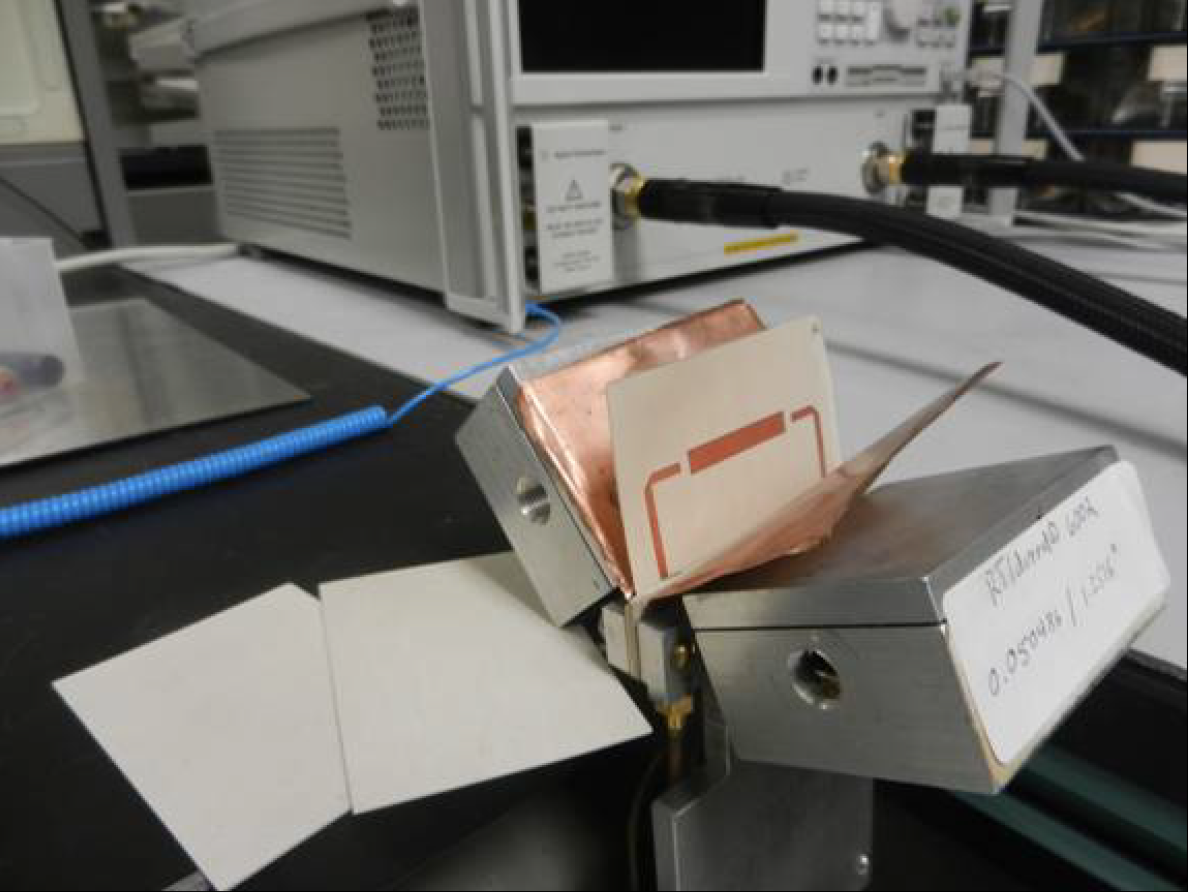
\includegraphics[width=10cm]{figures/tm2555c.png}};
    \draw [-latex, thick, green] (-0.75,6) node[anchor=east, black] {\small Clamp} to (4.5,3.5);
    \draw [-latex, thick, green] (-0.20,4) node[anchor=east, black] {\small Coupling strips} to (5.5,3);
    \draw [-latex, thick, green] (-0.5,2) node[anchor=east, black] {\small Specimens} to (0.5,1.8);
    \draw [-latex, thick, green] (10.75,6) node[anchor=west, black, text width=2cm] {\small Pattern card} to (6.5,4.5);
    \draw [-latex, thick, green] (10.3,4) node[anchor=west, black] {\small Copper sheets} to (7.5,3.75);
    \draw [-latex, thick, green] (10.75,1.5) node[anchor=west, black,text width=2cm] {\small Strip line resonator} to (6,3.75);
\end{tikzpicture}
\caption{Stripline resonator according to IPC TM-650 2.5.5.5c, adapted from \cite{horn}.}\label{fig:tm2555}
\end{figure}

Substrate and printed circuit board manufacturers often perform dielectric measurements, which are very important for the quality control in printed circuit board manufacturing and for the design of electronic circuits. The reason for this is that high-frequency electronics manufacturers need a consistent $\epsilon_r$ value for their production, which implies a tight $\epsilon_r$ control in PCB production. Horn \cite{horn} claimed that the $\epsilon_r$ of a substrate must not vary more than 0.5\% from batch-to-batch and within the sheet itself in order to meet customer requirements. He suggested that a measurement method with an relative accuracy for the $\epsilon_r$ of less than 0.5\% must chosen to measure these small variations in the dielectric substrates. As manufacturers are well experienced with printed circuit techniques, many of them use printed circuits for their dielectric measurement. Typically, they use one of the popular planar transmission lines like striplines, microstrips or co-planar transmission lines. These can be used in travelling-wave methods or standing-wave methods for planar circuits, but we will only discuss the standing-wave methods here as the former suffer from the same issues as other travelling-wave methods. Widely used standing-wave techniques are ring-resonators, T-resonator and strip\-line resonators. Especially the clamped stripline resonator of IPC standard IPC-TM-650 2.5.5.5c \cite{tm650} is widely used by PCB manufacturers and measurement results can be found in many datasheets. The method is illustrated in Fig. \ref{fig:tm2555}, two pieces of unclad substrate are sandwiched together with a thin strip of copper and two coupling strips in the middle, and are then pressed together by two pieces of copper at the top and the bottom. The result is a capacitively coupled strip line resonator, which allows quick and repeatable dielectric measurements that are excellent for quality control.

Planar circuit techniques have very genuine advantages, first of all the field orientation of the electric field in the substrate is the same as in a practical circuit. As single-ended planar transmission lines have one or multiple ground planes, the field orientation in the material is mostly perpendicular to the surface of the material. Combined with the fact that most PCB materials are weakly anisotropic, a measurement method that has the same field orientation as a circuit delivers the right dielectric constant for that circuit. Secondly, planar substrate techniques can include all loss mechanisms in a circuit - dielectric losses and conductor losses. As there are various types of copper claddings available on the market, measuring both loss mechanisms can deliver better predictions for the performance of a circuit as the entire system of copper cladding and dielectric is measured and not only the dielectric. For a PCB manufacturer these two are very important advantages, but these advantages pose serious challenges for dielectric measurements. In case of the field orientation, the orientation of planar circuits is not only perpendicular to the substrate, but there are also fringing fields that have field components parallel to the surface. The influence of fringing fields depends on the type of transmission line. Microstrips, for example, have far stronger fringing fields than strip lines, which can cause measurement errors in anisotropic materials. This makes microstrip resonators and transmission lines far less suitable for dielectric measurements. Another disadvantage of the perpendicular field orientation are potential systematic measurement errors that can be caused by air gaps, which can make a measurement method understate the dielectric constants of high-$\epsilon_r$ laminates.

For the loss measurements the situation is not much better, if we wanted to measure the dielectric losses of a material, we would have to separate the dielectric losses from the total losses in the material. As the conductor losses are typically far higher, there is a large uncertainty for the dielectric losses in the material. This makes substrate methods far less attractive for low-loss dielectrics. For example, according to NIST Technical Note 1520 \cite{tn1520} the ring-resonator and the T-resonator are limited to materials with a loss tangent $\tan\delta>\num{1e-3}$. Additionally the results of open structures like microstrip lines or co-planar strip lines may be affected by radiation losses. Impurities introduced by the manufacturing of the copper cladding may also change the dielectric properties. All in all, planar circuit methods are interesting options for approximate dielectric measurements of cladded printed circuit board substrates, since they offer the right field orientation in the substrate and they include most loss mechanisms in the material. For accurate dielectric measurements they should be used with utmost care, since systematic errors like airgaps, field orientation, anisotropy and conductor losses can negatively affect a measurement.
\section{Split-Post Dielectric Resonator Method}
\begin{figure}
\centering
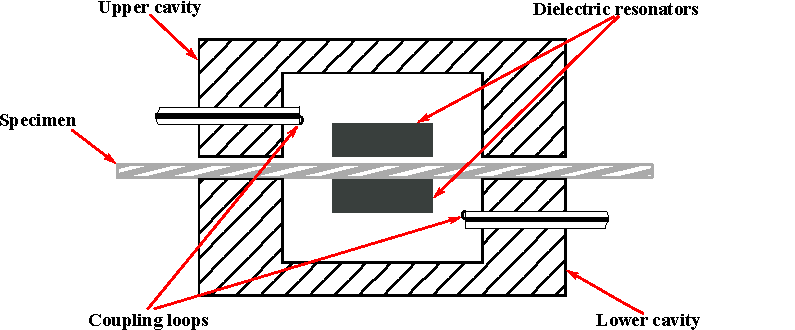
\includegraphics[width=0.8\textwidth]{split_post_dielectric_resonator.pdf}
\caption{Split-post dielectric resonator.}\label{fig:split_dr}
\end{figure}

The second standing wave method that we would like to discuss here, the split-post dielectric resonator method, bears many similarities to the split-cylinder method and other TE\st{0n} mode cavities. It was developed by Krupka, Nishikawa and DelaBalle \cite{dellaballe,nishikawa,krupka} in the 1980s and is one of the easiest and most convenient methods for measuring dielectric properties. It has become an industry standard for the measurement of PCB laminates and dielectric substrate \cite{iecSPDR}. Figure \ref{fig:split_dr} illustrates the geometry of a split-post dielectric resonator. The resonator consists of two cylindrical microwave cavities that both have a dielectric resonator placed along the z-axis of the cavity. One half is placed above the other with a small gap still separating the two halves. The resonator is then excited by coupling loops inserted into the bottom cavity and the top cavity. When the resonator is excited, the two dielectric bricks in the cavity experience a coupled TE\st{01$\delta$} resonance and the two resonators are coupled by evanescent fields. Unlike the evanescent fields of a single resonator, the evanescent fields between the two dielectric resonators are relatively strong. Dielectric specimens can therefore be placed in the gap between the two cavities and perturb the resonance of the resonator. Again, we can use the perturbation of the resonator to measure the complex permittivity of the specimen \cite{NPL, janezicSPDR, krupka}.

Since most of the electro-magnetic energy is stored in the dielectric resonators and in the region between the two resonators, there is far less interaction with the cavity walls than in a typical cavity method. This allows the split-post dielectric resonator to have a far greater sensitivity for dielectric loss measurements and resolutions as low as \num{2e-5} for $\tan\delta$ may be achieved. Split-posts dielectric resonators can be manufactured in a frequency range from \SIrange{1}{36}{\giga\hertz}, but they only operate at a single frequency. Their advantage over other cavity methods is that the frequency shifts of Split-post dielectric resonators are generally smaller and that the measurement frequencies for different specimens are roughly the same - a cavity may be detuned by a specimen as much as \SI{3}{\giga\hertz}! Like TE\st{0n} mode cavities, the evanescent field is also circularly polarised and therefore continuous across air-dielectric interfaces. This mitigates the influence of airgaps and allows the operator to measure thin films and coatings \cite{NPL, janezicSPDR, krupka}.

Although the resonator has many advantages, there are a few downsides: First of all, the modelling of the split-post dielectric resonator is far more complicated than other dielectric measurement methods. There are no analytical models, so numerical techniques like mode-matching, finite-difference, finite-element or Rayleigh-Ritz methods must be employed. Although it is very similar to perturbation methods, it cannot be modelled using perturbation methods. Secondly, their are restrictions on the thickness of the specimens. Specimens can only be as thick as to allow strong coupling between the two resonators. At higher frequencies decoupling issues are more likely, so even thinner specimens may be required. Lastly, the technique is not usable at millimetre frequencies and becomes increasingly hard to use above \SI{10}{\giga\hertz}. At these frequencies cavities have to be very small and the thickness of the specimens is very limited, so split-post dielectric resonators are typically used from 1-\SI{10}{\giga\hertz}. Overall, the split-post dielectric resonator method is an excellent method for measuring thin, low-loss dielectrics in the 1-\SI{10}{\giga\hertz} frequency range. The dielectric constant of thin specimens can be measured with an accuracy of less than $\pm 0.3\%$ and the resolution of the loss tangent measurements may be as small as \num{2e-5}, although these figures may be worse for thicker specimens \cite{NPL, janezicSPDR, krupka}.
\section{Open-Resonator Methods}
\begin{figure}
\centering
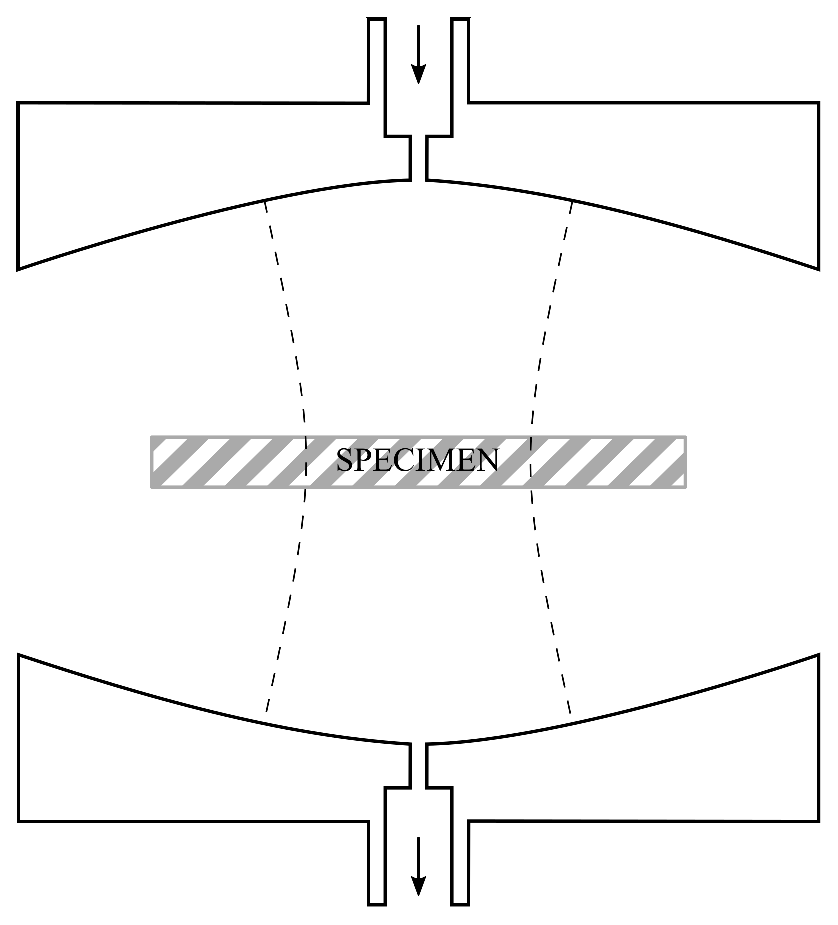
\includegraphics[width=0.4\textwidth]{open_resonator.eps}
\caption{Open resonator with two concave mirrors coupled to waveguides, adapted from \cite{NPL}.}\label{fig:or}
\end{figure}

At millimetre wave frequencies many methods become less practicable. Cavities for example become inconveniently small as their sizes are usually proportional to the wavelength $\lambda$. At these frequencies quasi-optical techniques like the open resonator method are used very often. An open resonator is a microwave Fabry-Perot interferometer, which uses two mirrors to focus electromagnetic waves in between these mirrors. A specimen is then placed between the  mirrors and, like for all other standing wave methods, the quality factor and the resonant frequency of the cavity are used to measure the complex permittivity of a specimen at the resonant frequencies. Different variants of the method exist and they can measure specimens over a wide frequency range 10-\SI{200}{\giga\hertz}. According to NPL \cite{NPL} it is one of the most accurate and important methods for low-loss dielectrics at millimetre-wave frequencies. It allows measuring the dielectric constant with an uncertainty of $\pm 0.2\% $ for $\epsilon_r < 3$, $\pm 1\% $ for $\epsilon_r\approx 50$ and the loss tangent with an uncertainty of $\pm 10\%$ for $\tan\delta >\num{2e-4}$. The measurement modes of the cavity are TEM\st{00n} Gaussian beam modes, so the electromagnetic waves in the cavity are focussed to a beam like in an optical resonator. The field orientation of the electric field varies over the beam length, so the placement of a specimen along the beam length would influence the measurement. To circumvent this, the sample is typically placed at the beam waist, where the field is nearly linearly polarised. This allows the open resonator method to measure in-plane anisotropy of a specimen just by rotating the specimen in the beam \cite{NPL,chen}.

Compared to other methods, the method has a few very unique advantages. First of all, like any free field method it allows easy insertion and removal of specimens, which do not have to be machined into certain shapes like for the measurements in a cavity. Typically, large sheet specimens are used that are large enough to encompass the whole cross-section of the Gaussian beam. As the beam width depends on the frequency different specimens sizes are required at different frequencies. At \SI{10}{\giga\hertz}, for example, specimens can be as large as 200mm, whereas at \SI{72}{\giga\hertz} a specimen may be as small as 35mm. Apart from the size, specimens should be reasonably flat and composite materials should be checked for high-$\epsilon_r$ filling materials as these can cause an scattering error in the measurement. Certainly, frequencies far lower than \SI{10}{\giga\hertz} are less attractive for the open resonator method and at these frequencies microwave cavities are usually preferred. Another advantage of the method are the high quality factors of its resonances, which are about 60,000 at \SI{10}{\giga\hertz} and can reach 200,000 at \SI{100}{\giga\hertz} and above. Together with a far less densely populated resonance spectrum, typical issues of microwave cavities like mode-coincidence and mode-interference are far less common. The quality factor of cavities on the other hand is proportional to $\lambda^{3/2}$, since losses increase with higher frequencies. Specimen losses grow slowly, so the sensitivity of cavity methods falls with higher frequencies. Higher modes in cavities have higher quality factors, but the number of modes grows with frequency and mode interference becomes an issue. This is also an essential advantage of open resonators, while the number of modes in an open resonator is proportional to the length $(L/\lambda)$, it is proportional to the volume $(L/\lambda)^3$ in cavities. Open resonators can be large, but the mode separation is still far better than in comparable cavities. All things considered, the open resonator method is a very versatile standing wave method, which can accurately measure the complex permittivity at microwave frequencies. The large frequency range, the ability to measure the anisotropy of a specimen and its good mode separation make it indispensable measurement method \cite{NPL,chen}.


 
